\section{Experiments}

\subsection{Training Data}
To train our model we use a subset of the dataset provided by the \gls{stc} as well as the ArchiMob corpus. The \gls{stc} provides two different datasets. An unlabelled dataset of about 300 hours spoken Swiss German. The labeled dataset contains mostly the Bernese dialect. An additional 1200 hours of unlabeled spoken Swiss German audio data. The unlabelled dataset includes mostly the Zurich dialect. Due to time limitations, we did not use the second provided dataset. We remove all audio files from the \gls{stcd} where the quality of the translation is rated lower than 0.7 (rating provided by \gls{stc}) which are still around 130k files. Additionally, we also need to remove files larger than 1 MB due to memory limitations (ca. 7k files). All files were converted from FLAC to Wav files and the sample rate was reduced from 48'000 Hz to 16'000 Hz to match the DeepSpeech input requirements. The official test set contains 13 hours of data \cite{stc2019} and has a dialect distribution conforming to the actual Swiss German dialect distribution. In addition to the official datasets, we used the ArchiMob corpus (Release 2) which contains 57 hours of spoken Swiss German data \cite{archimob2016}. They provide Swiss German and German transcriptions and it consists of various different dialects.
The German DeepSpeech comes with a script to pre-process the transcriptions. The pre-processing includes:
\begin{itemize}
\item removing of all unallowed characters (allowed are a-zA-Zäüö)
\item convert special characters like \$ to their written form (i.e. dollar)
\item convert numbers to their written form
\item lowercase
\item map all character with diacritics to one of the allowed characters
\end{itemize}

This fits the requirements given by the \gls{stc}.

\subsection{Evaluation metrics}
We evaluate our model through two types of metrics. The BLEU score \cite{Papineni2002BleuAM}, which is required by the \gls{stc} to compare the results. The \gls{stc} specifically requires a corpus-based BLEU score, which aims at measuring the distance/similarity of the generated text and the provided ground truth. As the German DeepSpeech test script does not include the BLEU score we added it manually. \\~\\Additionally, we keep track of the \gls{wer} for our models, as
this is a common metric for speech recognition systems \cite{Park2008AnEA} which is also included in the German DeepSpeech.

\subsection{Environment}
We train the model on a single NVIDIA GeForce RTX 2070 Laptop GPU (8 GB memory). We perform minimal tuning of our model's hyperparameters following the work of \newcite{Agarwal2020LTLUDEAL}.
.

\subsection{Models}
Following \newcite{Agarwal2020LTLUDEAL} we use a DeepSpeech architecture \cite{Hannun2014DeepSS} as our main model for speech-to-text translation. In order to get better results we use a
pre-trained DeepSpeech model \cite{DeepSpeechGerman090} as the base model for most of our experiments. The first model we trained served as our private baseline. \paragraph{Baseline model} We trained a bare DeepSpeech model with the default DeepSpeech hyperparameters on the labeled \gls{stcd} which achieved a BLEU score of 0.13 on our internal test set. The baseline model will be referred to as the baseline model or model \#0 henceforth.
\paragraph{Pre-trained model \#1} In order to improve our baseline model we use a pre-trained
German DeepSpeech model \cite{DeepSpeechGerman090}, which is fine-tuned on the \gls{stcd} dataset. We used \citet{Agarwal2020LTLUDEAL} best-reported hyperparameters which are learning rate of 0.0001, dropout of 0.25. The alpha and beta values for the language model are 0.40 and 1.10 respectively. We continue to use these hyperparameters as those provided better results. The model achieved a BLEU score of
0.23 on the validation set and 0.0004 on the official test set.
\paragraph{ArchiMob data model \#2} As the \nth{1} model did not achieve the expected results we decided to fine-tune our model on the ArchiMob data, as we expected the data distribution to be closer
to the actual test set. We trained for another 30 epochs with the same hyperparameters as in model \#1. We achieved the following BLEU scores for the validation and test set, 0.27, 0.17,
respectively.
\paragraph{Augmented data model \#3} In order to produce a more robust model, that can handle different pronunciations and speeds, we added data augmentation to our \nth{2} model. We fine-tuned our
model with the following data augmentations:
\begin{itemize}
    \item warp: ''Applies a non-linear image warp to the spectrogram. This is achieved by randomly shifting a grid of equally distributed warp points along the time and frequency axis''
    \cite{DeepSpeechAugmentation}
    \item tempo: ''Scales spectrogram on the time axis and thus changes playback tempo.'' \cite{DeepSpeechAugmentation}
\end{itemize}

The \gls{stcd} dataset is used for the augmentation fine-tuning on the \nth{3} model. This approach achieved a BLEU score of 0.28 on the validation set and 0.1 on the test set. The model was trained for another
20 epochs with a warp probability of 0.1 and a tempo probability of 0.1. One epoch on this model took around 3.5h to complete. Due to time limitations we
were not able to continue training the model any further, but the model was still improving and we expect that this approach could produce even better results. The \gls{wer} progression is depicted in the following plot:
\begin{figure}[H]
    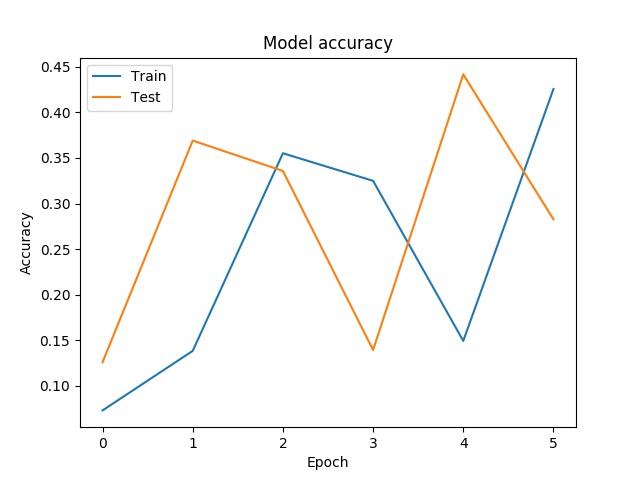
\includegraphics[width=\linewidth,height=5cm]{img/werPlot.png}
    \caption{WER per epoch}
    \label{fig:werPerEpoch}
\end{figure}

\paragraph{Text-to-Text model \#4} Our \nth{4} approach tries to improve the output by adding a text-to-text translation model after the speech-to-text model. We fine-tuned a pre-trained German to
English model following \newcite{TiedemannThottingal:EAMT2020} using the ''huggingface'' framework \cite{wolf-etal-2020-transformers} on the \gls{stcd} dataset. With this approach we achieved a BLEU score of 0.13 on the validation dataset and
0.07 on the test dataset.
